
\subsection*{Рабочие формулы}
    Формула дифракции Фраунгофера:
    \begin{equation}\label{eq::fraung}
        \frac{\lambda}{D} = \frac{\Delta x}{L}
    \end{equation}
    где $\lambda$ -- длина волны, $D$ -- цена деления шкалы,
    $\Delta x$ -- расстояние между дифракционными максимумами на экране,
    $L$ -- расстояние от шкалы до экрана.

    Формула тонкой линзы:
    \begin{equation}\label{eq::thin_lense}
        \frac{1}{a} + \frac{1}{b} = \frac{1}{F}
    \end{equation}
    где $a$ -- расстояние до источника (со знаком),
    $b$ -- расстояние до изображения (со знаком),
    $F$ -- фокусное расстояние.
 

    Радиусы колец голограммы точечного источника:
    \begin{equation}\label{eq::rad}
        r = \sqrt{m \lambda d}
    \end{equation}
    где $r$ -- радиус кольца, $m$ -- номер кольца, $\lambda$ --  длина волны,
    $d$ -- расстояние от точечного источника до фотопластинки. 

\subsection{Изучение характеристик голограммы точечного источника}

    Предлагается рассчитать расстояние от голограммы до точечного 
    источника, использованного при её создании, двумя способами:
    \begin{enumerate}
        \item измерив радиусы голографических колец на экране, 
                полученных с помощью короткофокусной линзы.
        \item используя голограмму в качестве фокусирующей линзы, 
              измерить параметры проекционной установки.
    \end{enumerate}

    \subsubsection*{Определение цены деления предметной шкалы}

        Устанавливаем кассету с транспарантами вблизи лазера. Освещаем лучом лазера шкалу и 
        получаем на удалённом экране дифракционную картину, созданную крестообразной шкалой.

        По результатам измерений $\Delta x = (0.59 \pm 0.02)$ см, $L = (127.90 \pm 0.14)$ см.
        Значение $\lambda$ дано изначально, $\lambda = 532$ нм. 
        Из формулы \eqref{eq::fraung} находим цену деления: $D = \frac{\lambda \cdot L}{\Delta x} = (115 \pm 4)$ мкм.

        Теперь, используя линзу с фокусным расстоянием $F = 4.3$ см, определим 
        цену деления $D$ этой же шкалы. Получим в результате измерений:
        $a = (4.3 \pm 0.1)$ см, $b = (123.60 \pm 0.17)$ см.
        Отсюда вычислим увеличение полученной системы $\Gamma = (28.7 \pm 0.7)$.
        Зная, что $\Gamma = \frac{D'}{D}$, получаем $D = (93 \pm 17)$ мкм.

        Видим, что значения, полученные разными способами достаточно близки.
        Также, исходя из величины погрешностей, заключаем, что 
        Первый способ обладает более высокой точностью измерения.

    \subsubsection*{Определение расстояние от голограммы до точечного источника}

        Получим на экране голографические изображения колец, занесём резульаты 
        измерения их радиусов в таблицу:


        \import{src/}{table.tex}
        На основании табличных данных построим график $r^2 = f(m)$:
        \begin{figure}[h!]
            \center{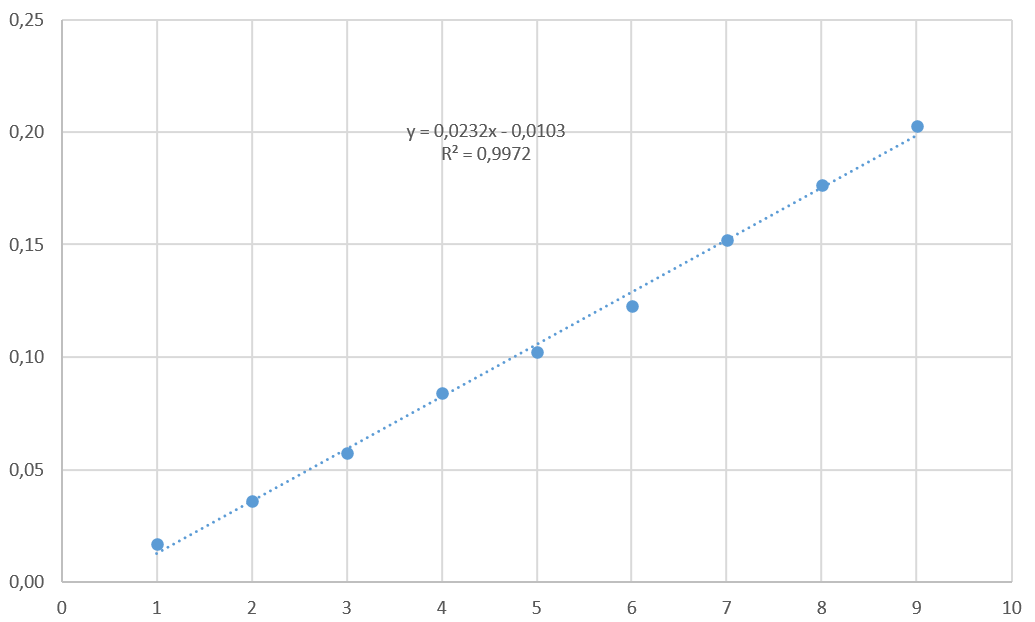
\includegraphics[width=0.9\linewidth]{graph.png}}
            \caption{График зависимости $r^2$ от $m$}
        \end{figure}

        Из формулы \eqref{eq::rad} получаем:
        $$
        r^2 = \lambda d m \Rightarrow r^2 \propto m
        $$
        то есть $r^2$ линейно зависит от $m$ с коэффициентом пропорциональности
        $k = \lambda d$. Из графика получим, что $k = (2.29 \pm 0.05) 10^{-2} \: мм^2$.
        Тогда получаем, что расстояние до точечного источника, который 
        использовался при создании голограммы равно $d = (43 \pm 1)$ мм.

        Перемещая линзу вдоль луча получаем на экране изображения мнимого источника $O_2$
        и действительного $O_3$. Зная фокусное расстояние лизны $F = 4$ см, а также 
        расстояние от лазера до каждого из изображений источников 
        $\rho(\text{Л}, O_2^*) = (2.3 \pm 0.1)$ см,
        $\rho(\text{Л}, O_3^*) = (8.8 \pm 0.1)$ см из формулы тонкой линзы: 
        \\
        $$
        \frac{1}{a} + \frac{1}{b} = \frac{1}{F}
        $$
        \\
        находим $\rho(\text{Л}, O_2) = (-5.4 \pm 0.6)$ см,
        $\rho(\text{Л}, O_3) = (7.3 \pm 0.3)$ см

    \subsubsection*{Изучение фокусирующих свойств голограммы}

        Добиваемся полного разделения пучков света на экране и определяем, какой из них соответствует действительному, какой мнимому изображению. 

        \noindent Установив перед голограммой предметную шкалу, получаем четкое изображение шкалы в пятне, соответствующем действительному изображению.
        
        \noindent Измерьте расстояние между штрихами $ \Delta x $ на экране и расстояние $L$ от экрана до голограммы. Используя эти данные, а также найденную ранее цену деления шкалы $D$, рассчитаем фокусное расстояние голографической линзы.
        
        \[ \Delta x = \frac{(9.5 \pm 0.5) \; мм}{7} = (1.36\pm 0.07) \; мм   ; \quad L = (510 \pm 5) \; мм \]
        \[ F = \dfrac{L}{1+\frac{D}{\Delta x}} = (4.6 \pm 0.1) \; см \]
        
\subsection{Изучение характеристик голограммы объемного предмета}
    \subsubsection*{Изучение мнимого изображения}
        
        \noindent Настроив систему и поместив голограмму в расширенный пучок лазера фотоэмульсией к лазеру находим мнимое изображение предмета. 
        $ \alpha = 32^o \pm 2^o $~--~угол поворота голограммы (угол падения опорного пучка).
        
        Постепенно закрываем голограмму листом бумаги и видим, что изображение почти не меняется, то есть восстанавливается не из полной картины.        
        На мнимом изображении видим линейку, а за ней стержень. На действительном изображении стержень расположен перед линейкой. 
        Оценим расстояние $h$ от линейки до вертикального стержня. Для этого рассмотрим отметку на линейке при разных углах поворота. Для угла $\alpha = 30^o$ при повороте на $\Delta \alpha =  10^o$ стержень соответствует делениям отстоящим на $l = 6$ мм. Тогда: \[h \approx \frac{l \cos \alpha}{\Delta \alpha} = 3 \; cm \]

    \subsection{Изучение действительного изображения}

        Находим действительное изображение, поворачиваем голограмму на $180^o$ вокруг вертикальной оси.
        Угол падения восстанавливающей волны, при которых возникает действительное изображение~--~$30^o$, мнимое изображение~--~$24^o$.
        Снова разворачиваем голограмму эмульсией к лазеру. Перемещаем короткофокусную линзу расширителя вдоль луча, наблюдаем, что при приближении линзы к лазеру изображение действительное увеличивается, мнимое уменьшается.
